\documentclass[10pt]{IEEEtran}
\pdfoutput=1

\usepackage{graphicx}
\usepackage{hyperref}
\usepackage[utf8]{inputenc}
\usepackage{listings}
\usepackage[table]{xcolor}
\usepackage{pdfpages}
\usepackage{algpseudocode}
\usepackage{natbib}
\usepackage{tikz}
\usetikzlibrary{shapes,shadows,arrows}

%style to be used on block diagrams
\tikzstyle{block} = [draw,rectangle, fill=white]
\tikzstyle{line} = [draw,thick]
\tikzstyle{arrowLine} = [draw,-stealth,thick]

%style to be used on flow charts diagrams
\tikzstyle{startstop} = [rectangle, rounded corners, minimum width=2.5cm,
minimum height=0.75cm,text centered, draw=black,fill=red!30]
\tikzstyle{io} = [trapezium, trapezium left angle=70,trapezium right angle=110,
minimum width=2.5cm,minimum height=0.75cm,text centered, draw=black,fill=blue!30]
\tikzstyle{process} = [rectangle, minimum width=2.25cm, minimum height=0.75cm, text centered, draw=black, fill=orange!30]
\tikzstyle{decision} = [diamond, minimum width=2cm, minimum height=0.5cm, 
text centered, draw=black,fill=green!30]
\tikzstyle{flowArrow} = [thick,->,->=stealth]


\hypersetup{colorlinks=true,citecolor=[rgb]{0,0.0,0}}


\title{Data mining with python: \\Automated FOREX trading}
\author{
	Kevin Voss Sjøbeck(s103451)\\
	\and
	Benjamin Maksuti(s103449)\\
	\and
	Anders Wessberg(s103477)
}


\begin{document}
\maketitle

\begin{abstract}
This project will utilize the oandapy API to get realtime data from the currency market to analyse, as well as enter and exit trades on based on the analytics. In the analytics we are going to use a short and a long moving averages, furthermore we are going to use MCAD as an extra precaution before we enter trades and use recovery zones to prevent losses on the account
\end{abstract}

\section{Introduction}
We all know the feeling about having money, but we also know the feeling of all the work we have to do in order of getting the money.
But what if you could have someone doing it for you? In this project we will try to make an automated trading bot. This bot will use oanda's API and in that way get a currency data and make trades on it.
For retrieving the data and making trades we will use machine learning with python, and in that way hopefully end out with some sort of profit.


\section{Analysis}

\subsection{Getting data}
We obtain all the financial data of the financial instrument EUR vs USD, on a 5 minute timeframe from oanda, using their own REST API for python. From oanda's API we get the financial charts of a 7 year time period, going from 2007-10-01 to 2014-10-20. After obtaining the data, it is stored in json fileformat in a file called "fxdata.txt", this data will then be used both to form our hypothosis of forex trading on the EUR vs USD currency pair, as well as performing a trading simulation on this set of data. However in order for us to use the naive Bayes classifier, we need to have two dataset's and not just a single one. In our domain the one dataset needs to be the trades which gained profit, and the other set needs consist of the trades which lost. We then have the possibility to analyze the data with different sets of features.\\
\\
The pseudo code of the random trading algorithm, where we will keep the orders for no more than 20 minutes:

\begin{center}
\begin{algorithmic}
\While{$streamFinancialData$}
	\State {$i = random(0,10)$}
	\If {$i = 0$}
    	\State {$openOrder(short)$}
	\ElsIf{$i = 1$}
    	\State $openOrder(long)$	    
	\EndIf
	\For{$order\: in\: orders$}	
		\If{$order.hasProfit()$}
			\State{$profitList.append(order)$}
			\State{$order.close()$}
		\ElsIf{$order.hasLoss()$}
			\State{$lossList.append(order)$}
			\State{$order.close()$}
		\ElsIf{$order.duration >= 4$}
			\State{$order.close()$}
		\Else
			\State{$order.duration += 1$}
		\EndIf
	\EndFor
\EndWhile
\State{$saveListToFile(profitList,"profit.txt")$}
\State{$saveListToFile(lossList,"loss.txt")$}
\end{algorithmic}
\end{center}

This algorithm should theoretically give us equally profitable trades in both the long and the short direction.

\subsection{Specific features}
To analyse the data we use a supervised classification learning algorithm, or to be more specific we use a naive Bayes classifier, the idea is to use a naive Bayes classifier on our financial data we gathered using our random algorithm. This isn't a new concept, in fact there are a couple of scientific articles on this already, as can be seen in the article by KAWABATA and TAKATA \cite{fxNaiveBayes}. We will train the classifier on some specific features accordingly to what the all powerful and knowing internet have told us would be a good idea to use to make strategies. One of the indicators many beginners are told to use are two moving averages, and when the functions cross it's an indicator to enter a trade, and also in what direction to enter the trade, the reasons why this is a good idea is explained in this video($https://www.youtube.com/watch?v=2_csKQ6iqx4$) from a website called "Financialtradingschool.com", he also explains about Price Action and how to use it in a strategy in the following video($https://www.youtube.com/watch?v=6FPfY1z1MyA$). So so far we know, that we should look at two SMA functions a slow and a fast, and look at when they cross. We also know that we should look at the prices directly in order to use it for Price Action, however since Price Action really is just a strategy to trade if the price reaches a certain point, we let our classifier doing the job, of defining when to trade or not directly based on the current prices of the currencies. Another indicator we found using the powerful internet was the relative strength index or the RSI indicator as it, is called in finance. Directly cited from http://www.investopedia.com/terms/r/rsi.asp("A technical momentum indicator that compares the magnitude of recent gains to recent losses in an attempt to determine overbought and oversold conditions of an asset."). This basically translate to, that if the RSI indicator gets to above 70 or above, it is a good indicator that you should make a short trade, and likewise if the RSI approaches 30 or below it is very likely a good idea to open a long trade. However we let our classifier determine whether it's a good idea to trade, depending on what the RSI level is directly. 
Due to our research on investment strategies our classifier should use the following features.

\begin{itemize}
	\item{CrossGraph(SMA(10,40))}
	\item{RSI(period=100)}
	\item{openBid(period=1)}
	\item{closeBid(period=1)}
	\item{volume(period=1)}
	\item{spread(period=1)}
	%\item{Parabolic SAR default settings (0.02, 0.2)}
	%\item{MACD default settings (fast=12, slow = 15, period=9)}
\end{itemize}


\begin{figure}
\begin{center}
	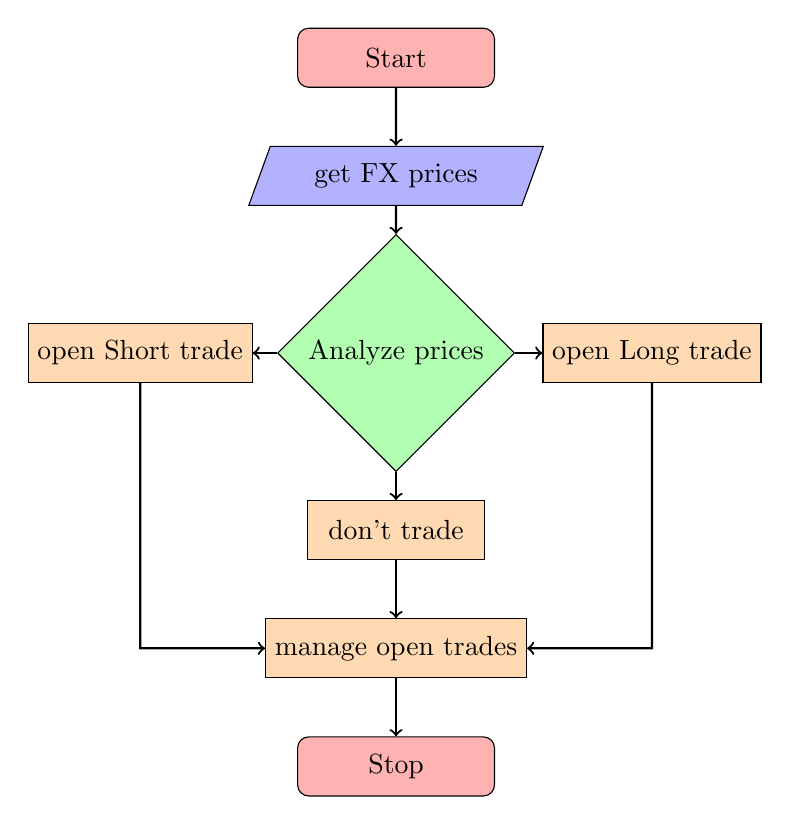
\begin{tikzpicture}[node distance=2cm]
		%blocks
		\node[startstop](start){Start};
		\node[io, below of=start,yshift=0.5cm](fx_price){get FX prices};
		\node[decision, below of=fx_price,yshift=-0.25cm](analyze){Analyze prices};	
		\node[process, right of=analyze, xshift=1.25cm](long){open Long trade};
		\node[process, left of=analyze, xshift=-1.25cm](short){open Short trade};
		\node[process, below of=analyze,yshift=-0.25cm](no_trade){don't trade};		
		\node[process, below of=no_trade,yshift=0.5cm](manage){manage open trades};				
		\node[startstop, below of=manage,yshift=0.5cm](stop){Stop};		
		
		%arrows			
		\draw[flowArrow](start)--(fx_price);
		\draw[flowArrow](fx_price)--(analyze);		
		\draw[flowArrow](analyze)--(long);		
		\draw[flowArrow](analyze)--(short);						
		\draw[flowArrow](analyze)--(no_trade);						
		\draw[flowArrow](no_trade)--(manage);
		\draw[flowArrow](short)--(-3.25,-7.5)--(manage);		
		\draw[flowArrow](long)--(3.25,-7.5)--(manage);		
		\draw[flowArrow](manage)--(stop);		
	\end{tikzpicture}
\end{center}
\caption{Flowchart of decision making}
\end{figure}


\section{Design}
Before we start trading, we need to train our classifier based on the feature set we mentioned in the analysis. After the training is completed, we can then start trading based on our historical data. 
After a completed run of the historical data, the result of the trade is then shown on a graph, showing the profit/loss of a 5 minute interval. Figure 1. is showing a flowchart of how the trading cycles. From this we know that we need a driver to run the program, that retrieves signals from either the Random trader or the classifier, depending on what is chosen. The driver then creates orders of trades, but to keep track of them all, we need an order manager. The driver also needs to be able to withdraw/deposit money to an account manager. Figure 2. is showing the class diagram on how we will implement it all.\\



\begin{figure}
\begin{center}
	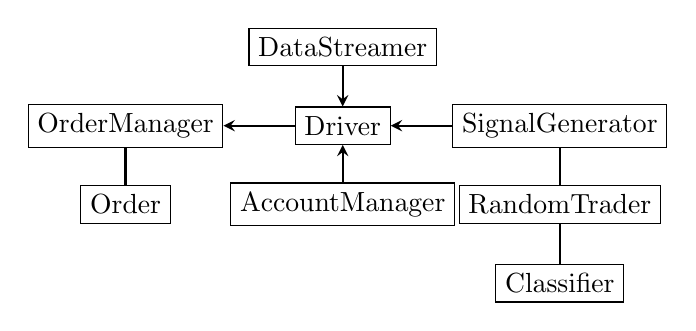
\begin{tikzpicture}
		\node[block](streamer){DataStreamer};
		\node[block,below of=streamer](driver){Driver};		
		\node[block,below of=driver](accountManager){AccountManager};				
		\node[block,left of=driver,xshift=-5em](orderManager){OrderManager};
		\node[block,below of=orderManager](order){Order};		
		\node[block,right of=driver,xshift=5em](signalGenerator){SignalGenerator};
		\node[block,below of=signalGenerator](random){RandomTrader};				
		\node[block,below of=random](Classifier){Classifier};						
		%arrows
		\path[arrowLine](streamer)--(driver);		
		\path[arrowLine](accountManager)--(driver);				
		\path[arrowLine](driver)--(orderManager);
		\path[line](orderManager)--(order);
		\path[arrowLine](signalGenerator)--(driver);
		\path[line](signalGenerator)--(random);				
		\path[line](random)--(Classifier);						
	\end{tikzpicture}
\end{center}
\caption{Overview of Classes}
\end{figure}




\section{Implementation}
\subsection{Order}
In the terminology of the FX market, an order contains all the relevant informations regarding the positions the trader opens. The information, that every order needs to have is the following.
\\
\\
the \textbf{required} is shown in bold
\begin{itemize}
\item{\textbf{units}}
\item{\textbf{side}}
\item{take profit}
\item{stop loss}
\item{duration or expatriation date}
\item{signals}
\end{itemize}

In addition to these properties the Order class does also contain the following methods.
\begin{itemize}
\item{check for close}
\item{close}
\end{itemize}

However we choose to save even more, we also store the signals the order was based on, this data will later be used by the classifier. 
In trading it's usually not enough to know, when it is smart to enter a trade. You also need to know when you should exit a trade, or to say it in terms of the FX market, you need to know when you should close your orders. In our implementation we do this by letting the order be set by some goals on the take profit, and stop loss and if the price ever reaches above or below those prices the order will return how much it's worth in the account currency. All the logic about when the order should be closed is happening in the check for close method. The close method is used to close the order right now. In other words, the check for close will only close the order if the order reaches it take profit or stop losses points or if it has reached it expiration date.
One thing that is very important to stress is that every time we close an order we take the spread into consideration and sell or buy at the lowest price. The way that we take the spread into consideration is that we buy at the highest available price, and sell at the lowest available price.

\subsection{Order Manager}
Our order manager is the main part of our system, not only does it keep a hold on every order and updates the orders with the newest price information on the currency pair, in order to check the orders if they should be closed or not. It also builds signals based on it's record of the 100 latest candles of price information. Furthermore this class is also responsible for the creation of orders, and while creating the orders make certain that the spread is taken into account, in the same way we do it, when the orders is closed by buying high, and selling low. A quick site-note regarding to the spread, is that the spread is often how the Brokers make their money, so the brokers don't care if we win or lose money on their platform as long as we keep trading, since the spread is almost like a tax on every \$ or euro you buy.

The class contains the following variables
\begin{itemize}
\item{account:AccountManager}
\item{leverage: Integer}
\item{profit: Double}
\item{orders: List}
\item{records: Dict}
\\
\\
\underline{The OCHLV data}
\item{open:List(100)}
\item{close:List(100)}
\item{high:List(100)}
\item{low:List(100)}
\item{volume:List(100)}
\end{itemize}

and it contains the following methods
\begin{itemize}
\item{update}
\\
This method checks if the open orders should be closed
\item{getSignals}\\
This method get the signals based on the current price candle
\item{crossingGraphs}\\
Test if two graphs cross each other, and gives a signal based  on their distance to each other in the y direction.
\item{createOrder}\\
This functions calls the account manager, and gets how many units should be opened for this position, and opens a trade corresponding to the side given as a parameter to the method.
\item{recordOrder}\\
This method is use to keep record of all of our previous trades.
\item{getClosedProfit}\\
This method return the accumulated profit based on all the closed orders
\item{getNrOpenOrders}\\
This method returns the number of open trades, this method is at the current time only used for debugging purposes, however it is easy to see that one could make a strategy, where no more than 5 orders should be opened at any time.
\item{closeAllTrades}\\
This method closes all open orders, we only use this method when we reach the last of our dataset, since it would be unfair to our algorithms if we had open orders, since we only use the closed profit as a parameter to see if we generate a profit.
\item{saveRecords}\\
This method saves all the records of the orders into two seperate files, one file for the profitable long trades, and another file for the profitable short trades, both of these files are saved in a JSON file format.
\end{itemize}


\subsection{Classifier}
In order to analyze our data we use a naive bayes classifier, and make the assumption that all of our features are independent despite coming from the same data source, this really ain't true, but if we take a short review of our choosen features we can clearly see that the majority of our features actually are independent. the volume, spread, openBid, RSI and even the evaluation of the two SMA graphs all of these features are independent of each other, in fact the only two features that depend on each other is the openBid and the closeBid. The naive baysian classifier is trained based on the following equation.
\\
\begin{center}
$ P(label|features) = \frac{P(label)*P(features|label)}{P(features)}$
\end{center}

In short for every feature there is certain probability of a specific label. This means that when the classifier classifies based on our features it uses the accumulated probability, it doesn't base it's 'guess' on the feature that has the highest probability.
However this way to calculate the probability can actually be used to our advantage, in such a way so we only open trades, when we have a confidence interval greater than a specified amount, in most statistics analyses the confidence interval chosen is 95\% however in our case we choose 96\% due to the reason, that we only want to open trades if we are really certain upon our guess.
The way we trade based on the classifier is that for every candle worth of data, we get the features of the latest FX data from the dataManager, according to these features we then let our classifier take an 'educated' guess, and if the classifier is more certain than the specified confidence interval it tells the dataManager to open a trade in the specified direction.

\section{Test \& Results}
\subsection{Test}
Our control test are made by running the program on the data.txt(roughly 23 days), with a leverage at 20, an account on 10000\$, and set the confidence level of the classifier at 96\%. When the program have gone though data, we retrieve the profit/loss. Hereafter we deviate one variable from the control, firstly we change the leverage to 400, then we change the confidence level of the classifier to 85\%.\\
We also want to check different datasets, the largest dataset goes from 2007 to 2014(, roughly 2557 days), then we use a data set that is newer than the control, going from 2014/11/10 - 2014/12/03(roughly 24 days) and the last data we go through is roughly a single day, the 2014/12/03, with a 5 second interval.\\
\\
We also test the random trader to see how effective it is, on both the control data and the large data FOOTNOTE The result may differ because the trade is random.\\
\\
We have generated graphs for each test, that shows the profit/loss on each interval, and the exchange rate for EUR/USD on each interval. FOOTNOTE See appendix for all graphs

Now that we have several test data, with the profit and by knowing how many days each data spanned over, we calculate the daily profit/loss for each test.
\subsection{Results}

\begin{tabular}{  l | c | c | c |}
\cline{2-4}
& Profit & Days & Profit/Days \\ \hline
\multicolumn{1}{ |c| }{Control data} & 357,18 & 23 & 15,53 \\ \hline
\multicolumn{1}{ |c| }{leverage=400} & 8974,66 & 23 & 390,20 \\ \hline
\multicolumn{1}{ |c| }{confidence=0.85} & 189,32 & 23 & 8,23 \\ \hline
\multicolumn{1}{ |c| }{Large data} & -7251,99 & 2557 & -2,84 \\ \hline
\multicolumn{1}{ |c| }{Newer data} & 31,54 & 24 & 1,31 \\ \hline
\multicolumn{1}{ |c| }{One day data} & 36,18 & 1 & 36,18 \\ \hline
\multicolumn{1}{ |c| }{One day data leverage=400} & 713,91 & 1 & 713,91 \\ \hline
\multicolumn{1}{ |c| }{Random Control} & -398,45 & 23 & -17,32 \\ \hline
\multicolumn{1}{ |c| }{Random Large} & -9998,00 & 2557 & -3,91 \\ \hline
\hline
\end{tabular}

\section{Discussion}

By changing some of the variables for the control data, we retrieve a result for the control data, one with the leverage on 400 and one with the confidence level on 85\%.\\
In these cases, the test with leverage on 400 gets the best result, even though we multiply the leverage with 20, the profit gained is more than 20 times the control(, it is 25 times more). This is due to that each time we make a trade we use 2\%, of the current account balance, which is capital projection. Changing the leverage creates a bigger risk, but might also improve the gain.\\
When we reduce the confidence level to 85\%, the classifier opens more trades, that have a higher risk, than with the leverage. This is duo to that you might get profit on more trades but the profit on each trade is closely the same, but duo to the higher risk you might also loose profit on more orders than earlier.\\
So if lowering the confidence level was a higher risk, then raising the confidence level will lower the risk. This is somewhat true, because raising the confidence level to high, only prevents the classifier of making any orders and therefore never trades.\\  
\begin{figure}[h]
    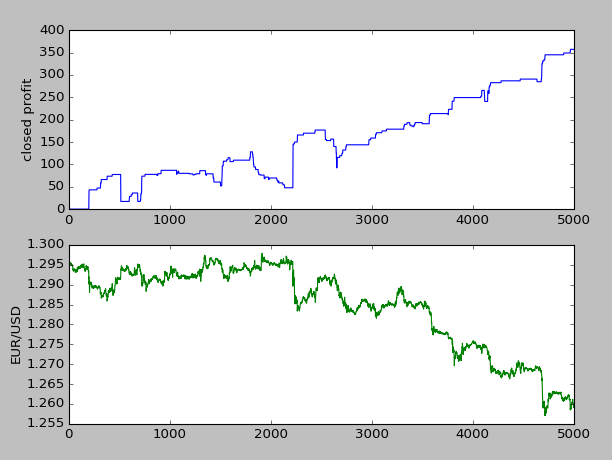
\includegraphics[scale = 0.5]{data-96-10000-20.png}
    \caption{This is a graph of the closed profit, on the control data.}
\end{figure}
\\
The next three result are where we keep the variables the same, but change the data we test on. So far we have had profit on each test, but with the large dataset, we get a closed profit of about -7250. Even though it might seem a lot, it is less than 3 dollars a day, spanning over 7 years. This shows that even with a confidence level on 96\%, you still might lose your money. By looking at the graph for the large data LINK TO GRAPH, we see that in the beginning, the classifier creates positive profit, but as we go on it looses. This might be because that we do not update the classifier each state.\\
\\
We therefore also made a test data, that was newer than both the large data and the control data. By looking at this graph LINK, we see that the classifier makes less trades, but also makes some larger mistakes. Even though we end in a profit with this data set, it is around 12 times less than in the control data. This confirms our theory that the classifier needs to be updated regularly to be able to work properly.
\\
\\
So far all our data have been collected over several day's, with a 5 min interval. We therefore decided to have a data set from a single day, with a 5 sec interval instead. This gave us the most profitable closed profit, at two times more than the control, a day.\\
\\
To see how well our classifier works, we use our Random trader with both the control data, and the larger data, these test represents how a normal person might trade. We ran these test several times, and not a single time did we end with a positive closed profit. This is quite expected, and also shows that without having knowledge of professional trader, or in our case having a bot trading for you.

\section{Conclusion}


Improvements:
A classifier that updates it self with newer data.
Using other features

\section{Terms \& abbrivations}
\begin{tabular}{l | l | l}
& Term or &\\
Domain & Abbreviation & Meaning\\
\hline
Trading & FX & Forex \\ 
Trading & Bid & An offer made by an investor,\\
& & a trader or a dealer to buy a security\\
Trading & Ask & The price a seller is willing to accept for a security\\
Trading & SMA & Simple Moving Average\\
Trading & MACD & Moving Average Convergence/Divergence\\
Trading & SAR & Parabolic SAR(Parabolic Stop and Reverse)\\
Machine Learning & NBC & Naive Bayes Classifiers\\
\end{tabular}


%plainnat
\bibliographystyle{plain}
\bibliography{roboFX}


\end{document}
